\section{Principal Component Analysis}

\begin{bigidea}
An $n \times p$ data matrix $X$ represents a set of $n$ samples in $\mathbb{R}^p$ and projecting the data onto the first $k$ principal components allows us to view the data in $\mathbb{R}^k$. Usually $k=2$ such that we can visualize the data in 2D.
\end{bigidea}

\begin{definition}
Let $\bs{x}_1 , \dots , \bs{x}_n \in \mathbb{R}^p$ (viewed as row vectors) and let $X$ be the $n \times p$ data matrix where row $k$ is given by $\bs{x}_k$. Assume the data is {\bf normalized} such that the mean value of each column of $X$ is 0. The unit vector $\bs{w}_1$ which maximizes the sum
$$
\sum_{i=1}^n \left( \bs{x}_i \cdot \bs{w}_1 \right)^2 = \| X \bs{w}_1 \|^2
$$
is called the {\bf first weight vector} of $X$ (see \href{https://en.wikipedia.org/wiki/Principal_component_analysis}{Wikipedia: Principal component analysis}). More generally, given weight vectors $\bs{w}_1 , \dots, \bs{w}_{k-1}$, the {\bf $k$th weight vector} of $X$ is the unit vector $\bs{w}_k$ which maximizes
$$
\| X_k \bs{w}_k \|^2
$$
where $X_k$ is the projection of the data matrix $X$ onto $\mathrm{span} \{ \bs{w}_1 , \dots, \bs{w}_{k-1} \}^{\perp}$
$$
X_k = X - \sum_{j=1}^{k-1} X \bs{w}_j \bs{w}_j^T
$$
The projection coefficient $\bs{x}_i \cdot \bs{w}_k$ is called the {\bf $k$th principal component} of a data vector $\bs{x}_i$.
\end{definition}

\begin{note}
Each $( \bs{x}_k \cdot \bs{w}_1 )^2$ is the length squared of the orthogonal projection of $\bs{x}_k$ onto $\bs{w}_1$. Therefore the first weight vector $\bs{w}_1$ points in the direction which captures the most information (ie.~the maximum variance) of the data, and the second weight vector $\bs{w}_2$ is orthogonal to $\bs{w}_1$.
\begin{center}
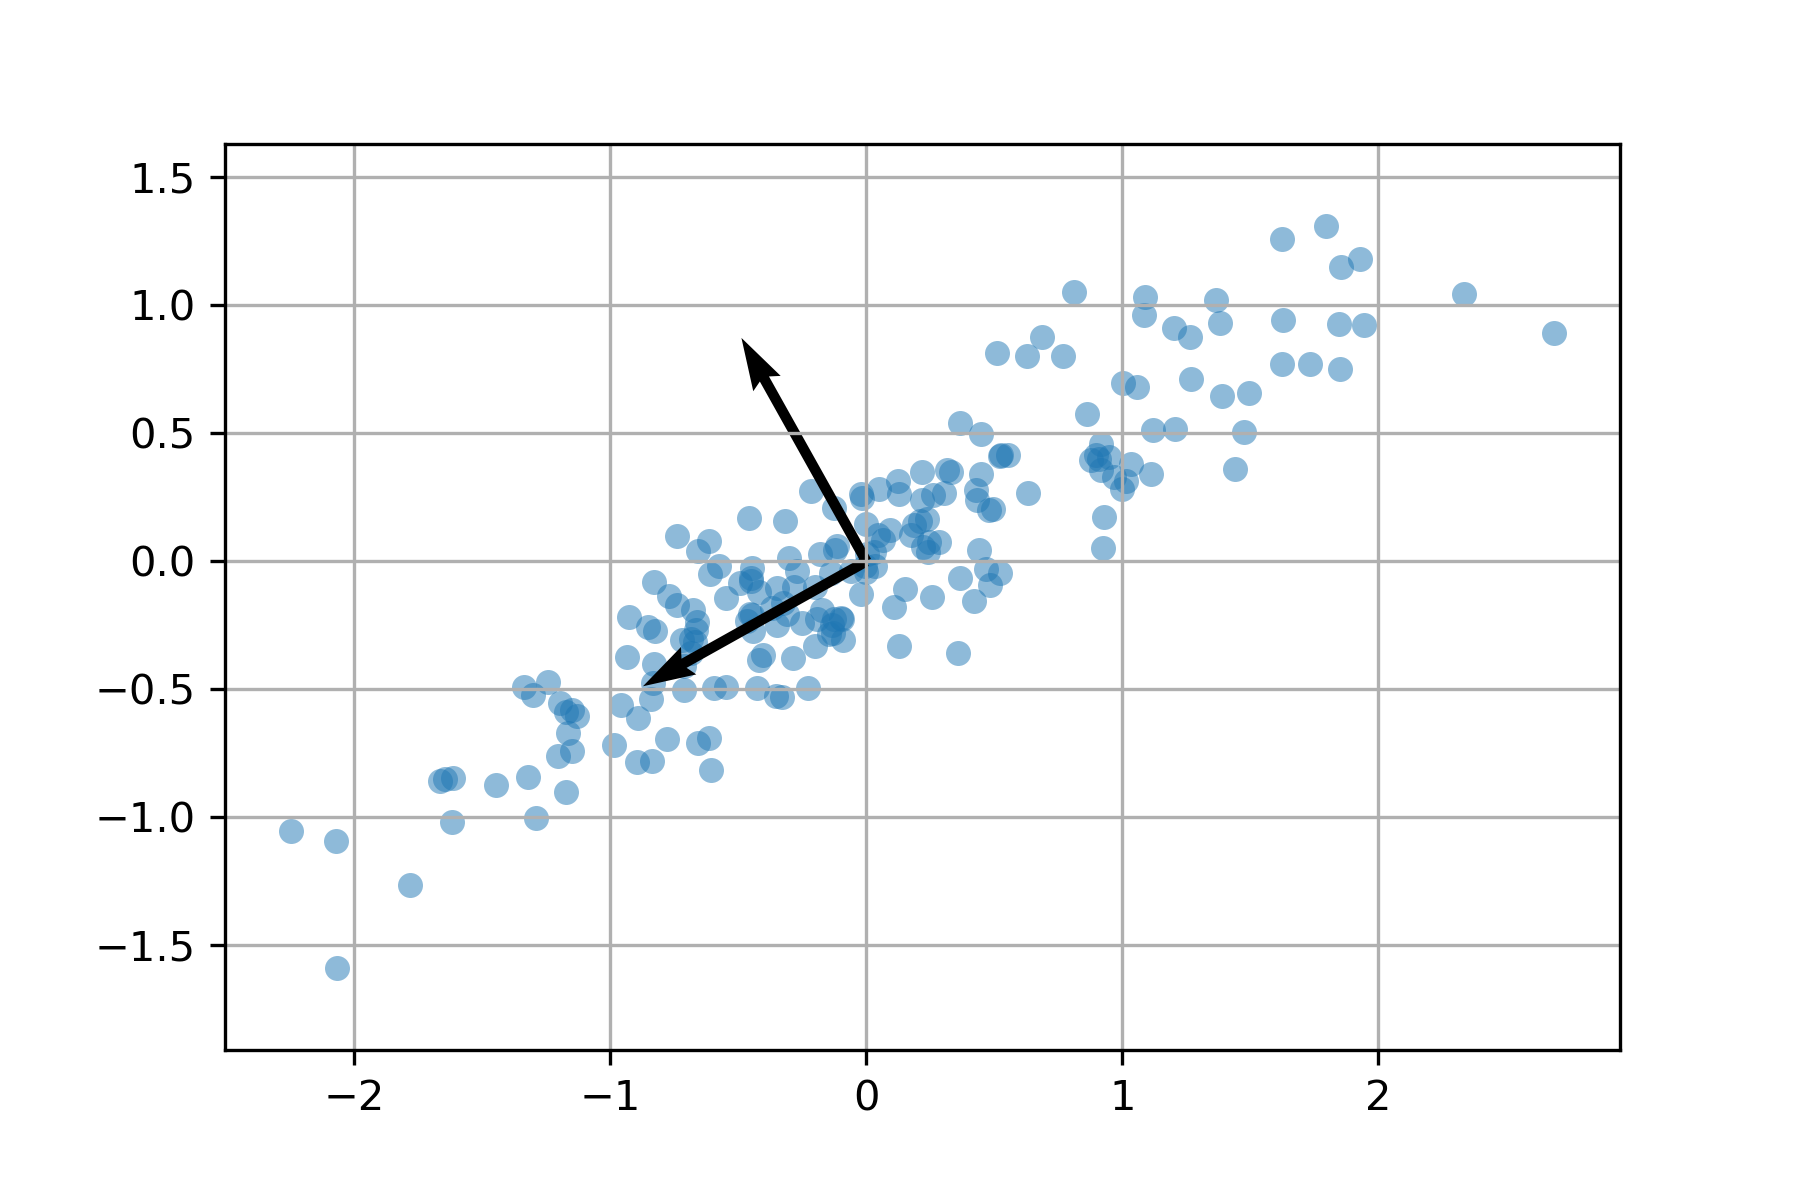
\includegraphics[width=3in]{03_04_img01.png}
\end{center}
\end{note}

\begin{proposition}
The weight vectors $\bs{w}_1 , \dots , \bs{w}_p$ are the right singular vectors of the matrix $X$. In other words, let $X = P \Sigma Q^T$ be a singular value decomposition of $X$ and let $\bs{q}_1, \dots, \bs{q}_p$ be the columns of $Q$ corresponding to singular values $\sigma_1 > \cdots > \sigma_p > 0$. Then $\bs{w}_1 = \bs{q}_1 , \dots , \bs{w}_p = \bs{q}_p$.

\begin{proof}
Let $X = P \Sigma Q^T$ be a singular value decomposition of $X$ and note
$$
\| X \bs{w} \|^2 = \| P \Sigma Q^T \bs{w} \|^2 = \| \Sigma Q^T \bs{w} \|^2
$$
since $P$ is orthogonal. Since $\Sigma$ is diagonal with diagonal entires $\sigma_1 > \cdots > \sigma_p$, the maximum value of $\| X \bs{w} \|^2$ occurs when $Q^T \bs{w} = \begin{bmatrix} 1 & 0 & \cdots & 0 \end{bmatrix}^T$ therefore $\bs{w}_1 = \bs{q}_1$. For general $k$, note that the singular value decomposition $X_k = P_k \Sigma_k Q^T_k$ is obtained from $X$ by removing the singular values $\sigma_1,\dots,\sigma_{k-1}$. Therefore the largest singular value of $X_k$ is $\sigma_k$ with corresponding right singular vector $\bs{q}_k$ and therefore $\bs{w}_k = \bs{q}_k$.
\end{proof}
\end{proposition}

\begin{example}
Find the first weight vector for the data given in the image below.
\begin{center}
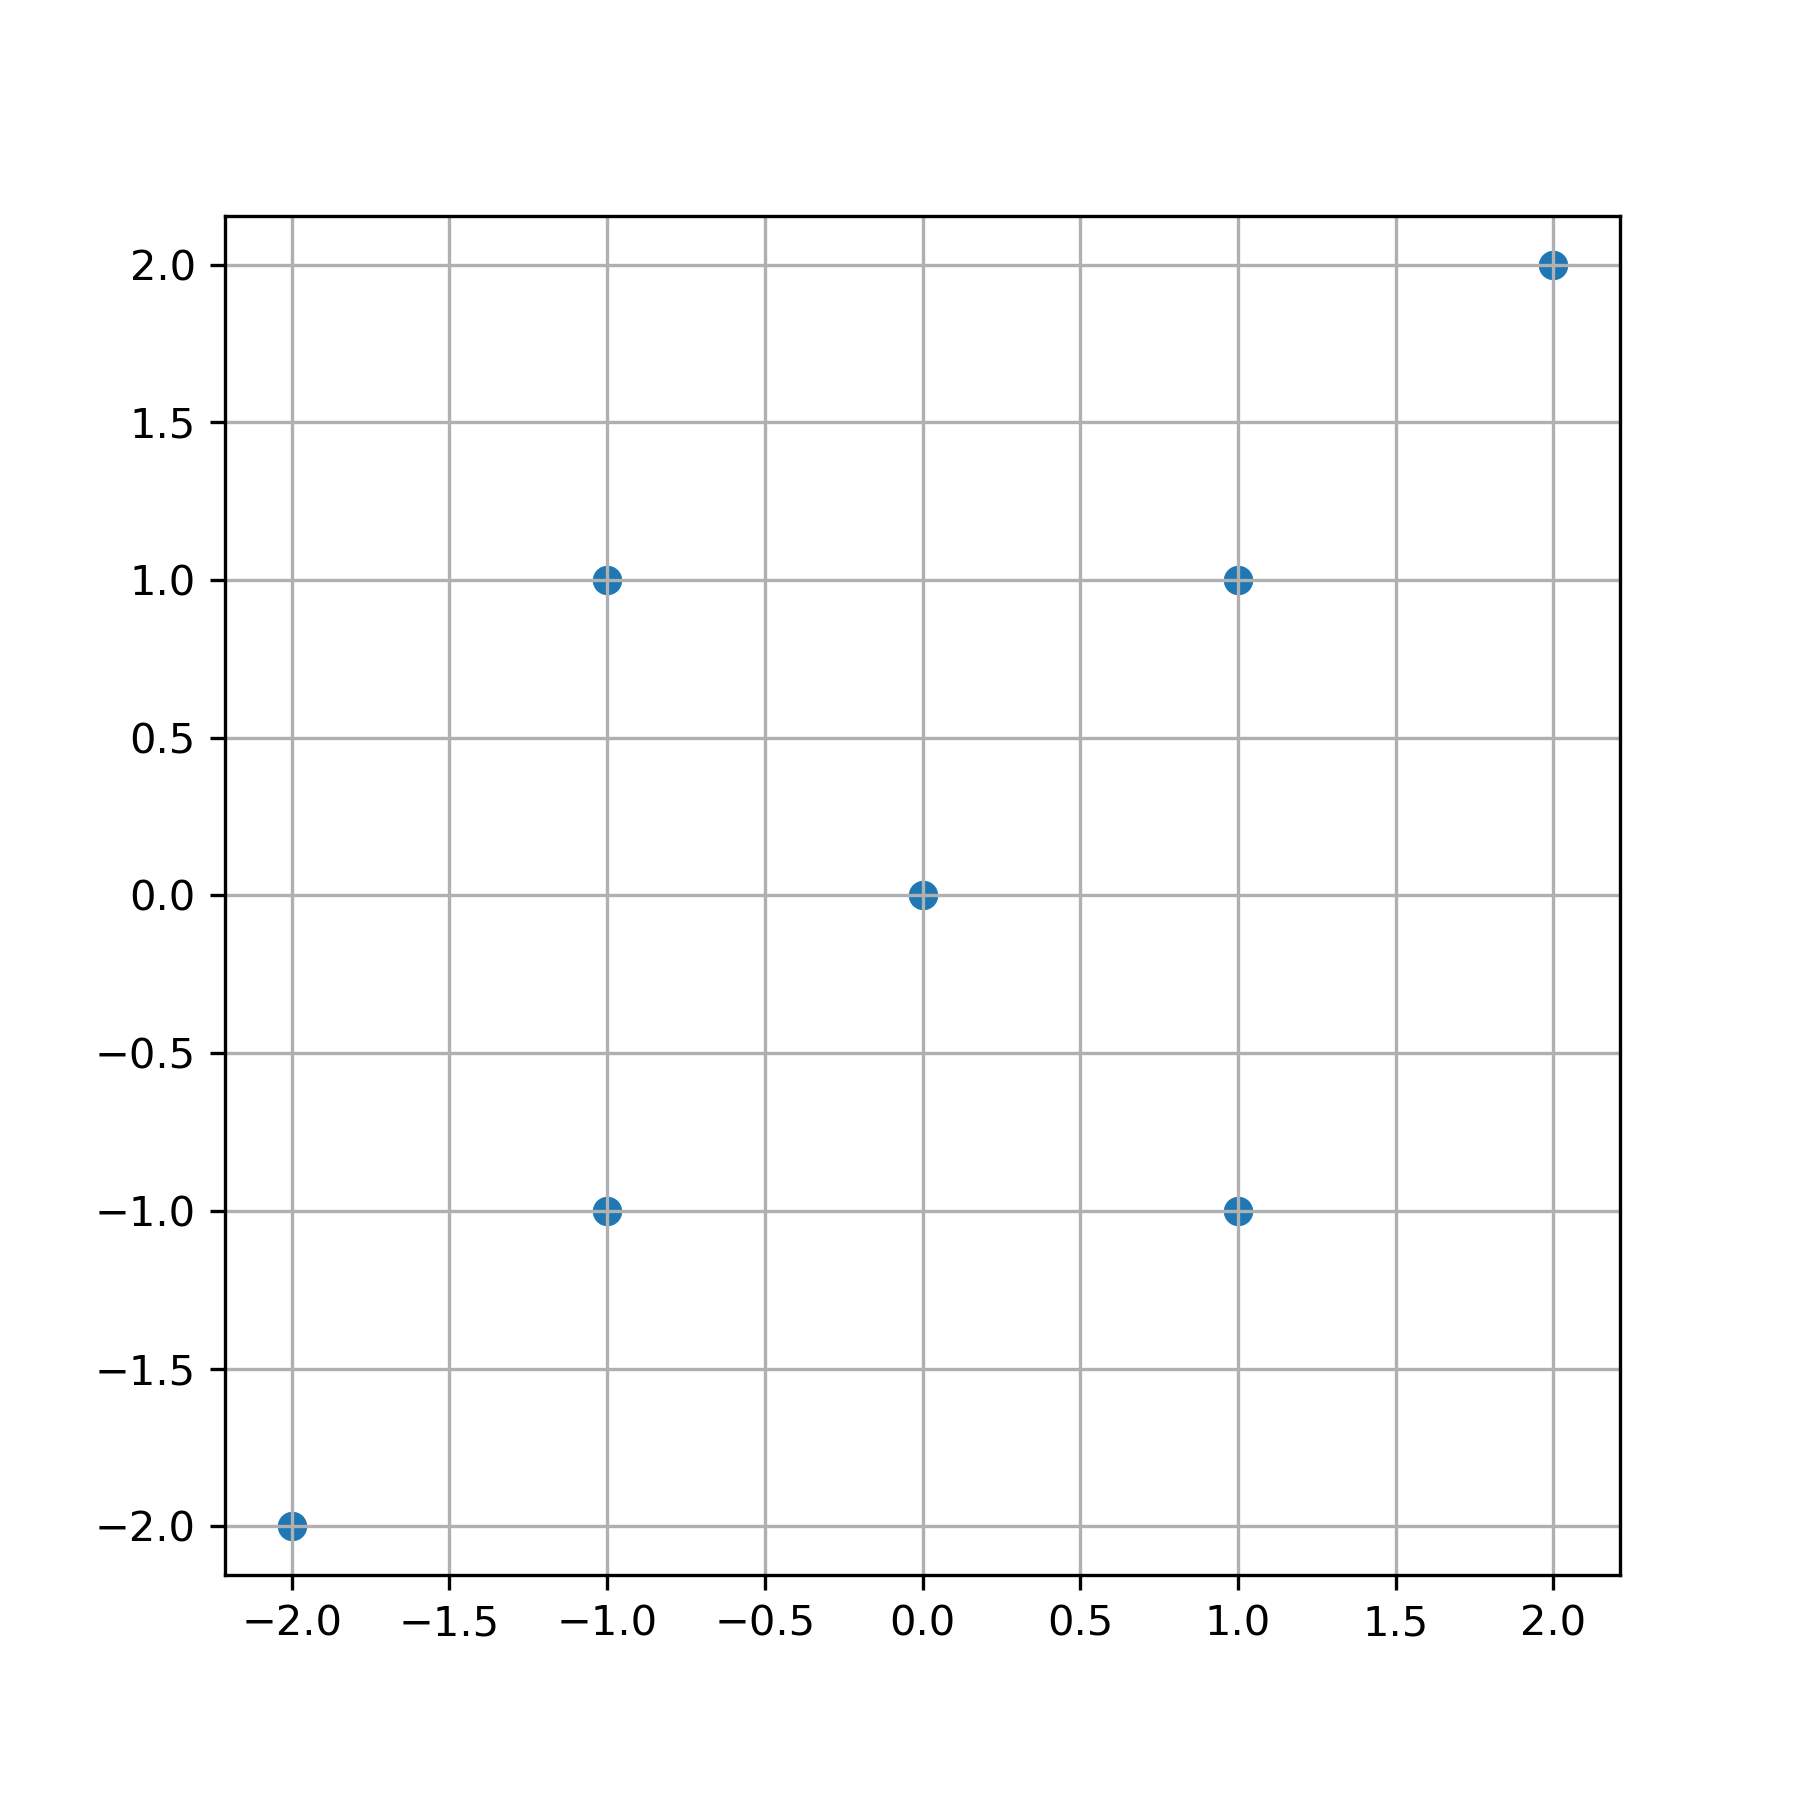
\includegraphics[width=3in]{03_04_img02.png}
\end{center}
We expect $\bs{w}_1 = \begin{bmatrix} 1/\sqrt{2} & 1/\sqrt{2} \end{bmatrix}^T$ since that direction clearly captures the most information. Form the data matrix
$$
X^T = \left[ \begin{array}{rrrrrrr} -2 & -1 & -1 & \phantom{+}0 & 1 & \phantom{+}1 & 2 \\ -2 & -1 & 1 & 0 & -1 & 1 & 2 \end{array} \right]
$$
We don't need to compute the full SVD of $X$ but just the first right singular vector. Compute
$$
X^T X = \begin{bmatrix} 12 & 8 \\ 8 & 12 \end{bmatrix}
$$
The characteristic polynomial of $X^TX$ is
$$
\det (xI - X^TX) = (x-12)^2 - 8^2 = x^2 - 24x + 80 = (x - 4)(x - 20)
$$
The right singular vector $\bs{q}_1$ for $X$ is a unit eigenvector for $X^TX$ for the eigenvalue $\lambda_1 = 20$. Compute
$$
( X^T X - 20 I)\bs{w}_1 = \bs{0} \ \ \Rightarrow \ \
\left[ \begin{array}{rr|r} -8 & 8 & 0 \\ 8 & -8 & \phantom{+}0 \end{array} \right]
 \ \ \Rightarrow \ \
 \bs{w}_1 = \frac{1}{\sqrt{2}} \begin{bmatrix} 1 \\ 1 \end{bmatrix}
$$
\end{example}

\begin{example}
The \href{https://scikit-learn.org/stable/modules/generated/sklearn.datasets.load_digits.html#sklearn.datasets.load_digits}{digits dataset from sklearn} is a $1797 \times 64$ data matrix $X$ such that each row represents an $8 \times 8$ pixel image of a handwritten number. The first 10 rows of X (reshaped from vectors of length 64 to $8 \times 8$ matrices to visualize) are:
\begin{center}
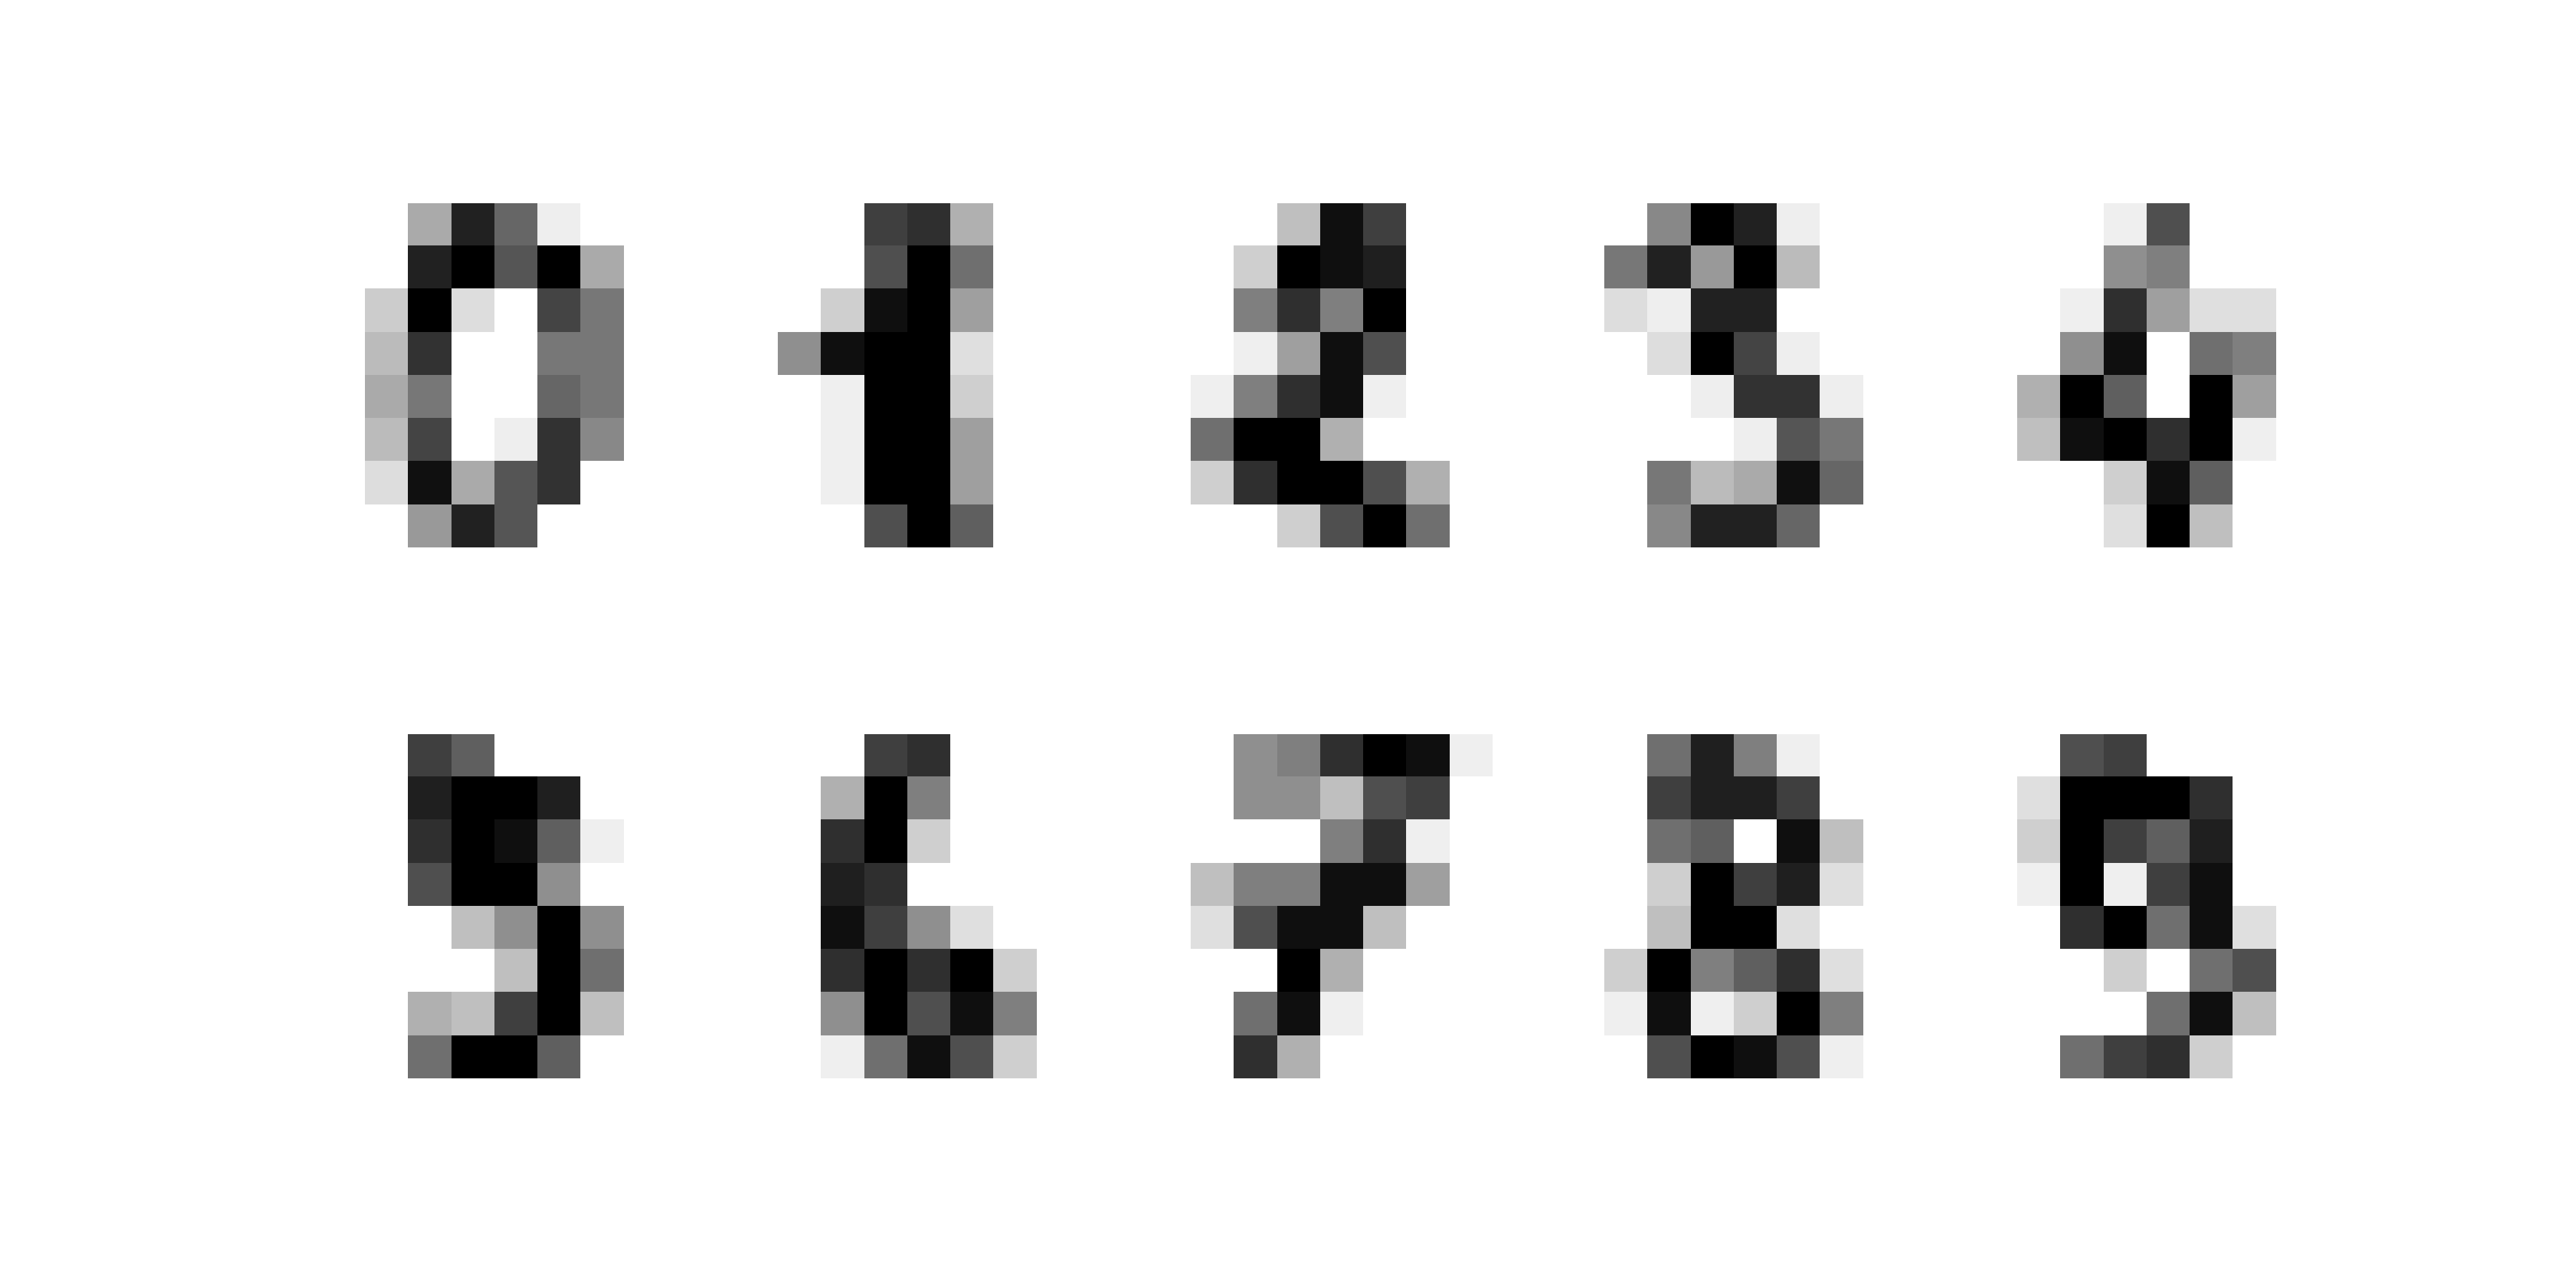
\includegraphics[width=3in]{03_04_img03.png}
\end{center}
Compute the first 2 weight vectors and find (again $\bs{w}_1,\bs{w}_2$ reshaped from vectors of length 64 to $8 \times 8$ matrices to visualize)
\begin{center}

\includegraphics[width=3in]{03_04_img04.png}
\end{center}
We can see $\bs{w}_1$ looks like a 3 and $\bs{w}_2$ looks like 0. Project the entire dataset onto these weight vectors and label each data point by a color according to the digit:
\begin{center}
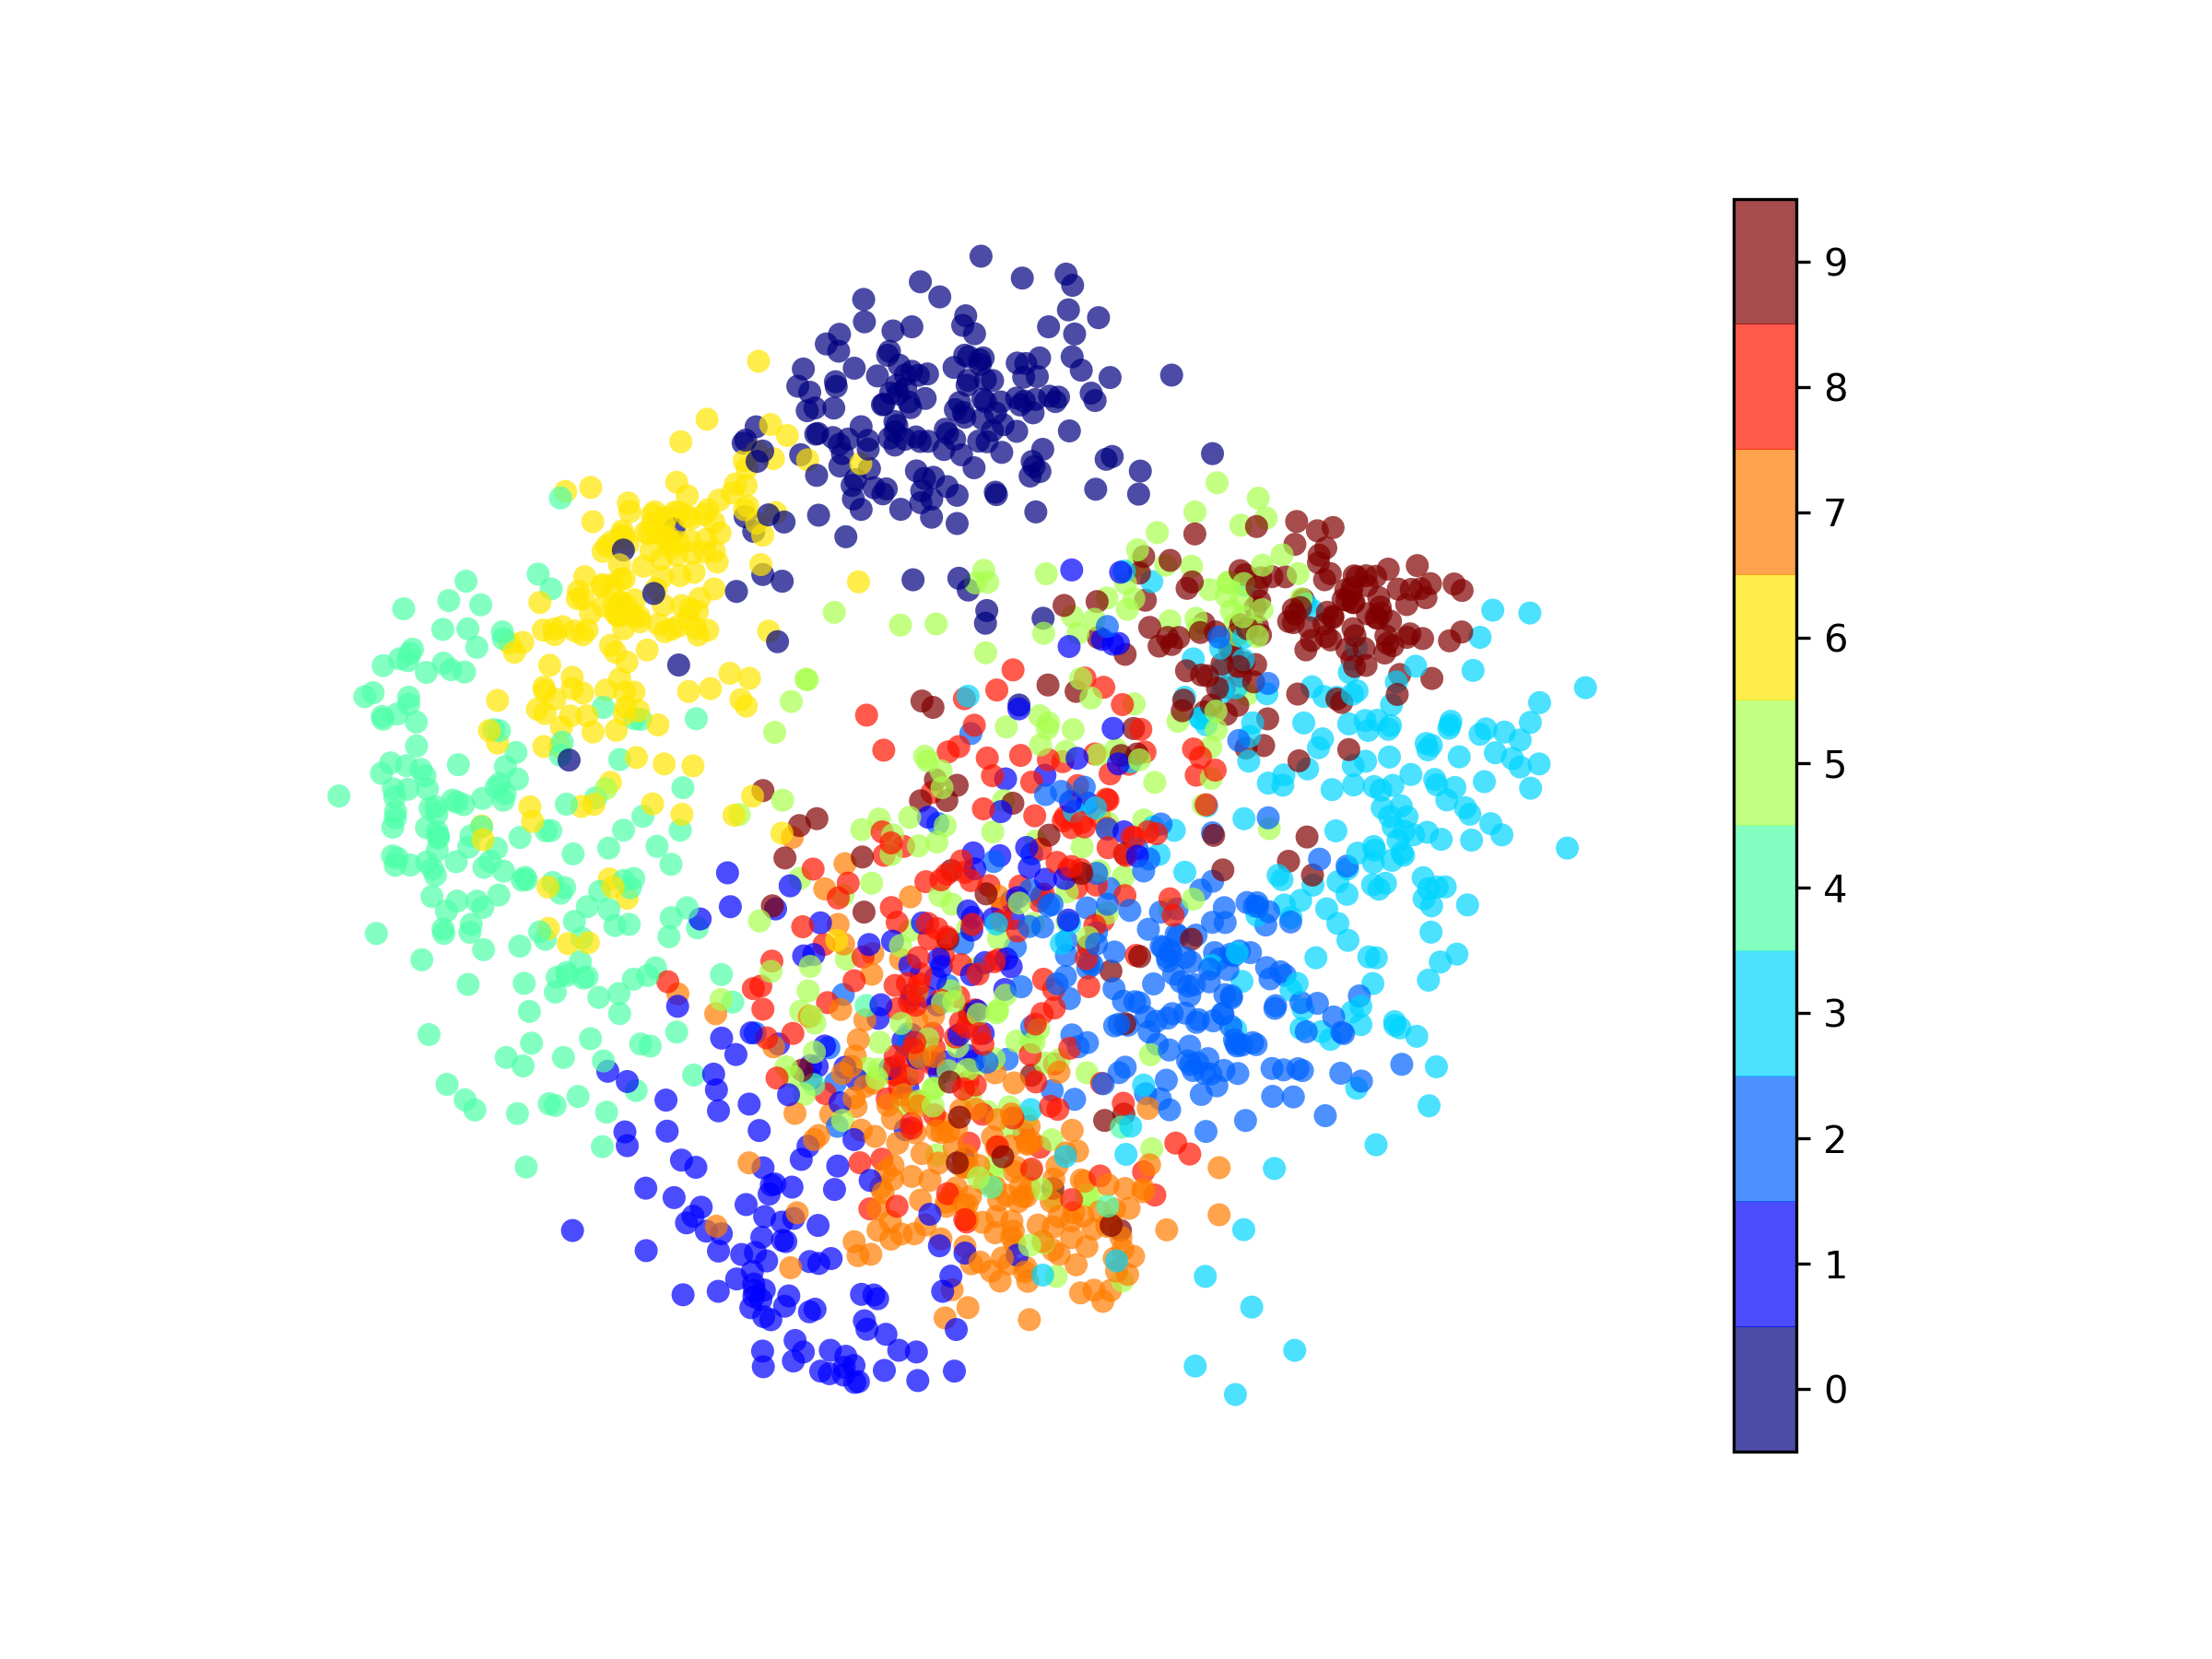
\includegraphics[width=4in]{03_04_img05.png}
\end{center}
We can see that the 3s are to the right in the horizontal direction since these points most similar to $\bs{w}_1$, and the 0s are at the top in the vertical direction since these points most similar to $\bs{w}_2$. We can make other interesting observations such as the 4s are opposite to the 3s and orthogonal to 0s, and 7s and 1s are opposite to 0s and orthogonal to 3s.
\end{example}